\documentclass[14pt]{extarticle}
\usepackage{amsthm,amsmath,amssymb,caption}
\usepackage[margin=0.5in]{geometry}
\usepackage[hidelinks]{hyperref}
\usepackage[draft]{graphicx}
\title{Renormalization group for interacting Fermions}
\author{Abhirup Mukherjee}
\begin{document}
\maketitle
\section{Summary of Renormalization Group}
The philosophy of the renormalization group approach is to integrate out high energy modes from a microscopic Hamiltonian and observe how the couplings morph in the process. This allows us to write down a low-energy effective Hamiltonian for the problem which can be used to describe low-energy excitations as well as universal features which depend on the short-distance details only through a small number of couplings which are, as a result, termed to be \textit{relevant}.

Say we have a free energy \(\mathcal{F}\), characterized by a scalar field \(\phi\). The partition function can be written as a path integral over all configurations of \(\phi_k\):
\begin{equation}\begin{aligned}
\label{oldpart}
Z = \int \mathcal{D}\phi \;\exp\left\{-\mathcal{F}(\phi)\right\}
\end{aligned}\end{equation}
where 
\begin{equation}\begin{aligned}
\mathcal{F}[\phi] = \int_0^\Lambda dk \;f[\phi(k)]
\end{aligned}\end{equation}
Let us assume there is a natural momentum cutoff in the problem \(\Lambda\). There are three distinct steps involved in the RG procedure:
\begin{itemize}
	\item Integrate out modes in the range \(\left[b\Lambda,\Lambda\right]\), where \(b < 1\).
	\item Rescale the momenta to keep the limits unchanged so that we can compare the new partition function with the previous one: \(k^\prime = \frac{k}{b}\)
	\item Rescale the fields so as to keep at least one term in the partition function unchanged (usually the Gaussian term) so that we can compare the changes in the rest of the terms: \(\phi^\prime = \lambda\phi\)
\end{itemize}

In a single iteration of the RG, the first step is to reduce the cutoff to \(b\Lambda\), \(b\) obviously being less than 1. To facilitate this, we separate the fields into high momentum and low momentum parts:
\begin{equation}\begin{aligned}
\phi(k) = \phi^<(k) + \phi^>(k)
\end{aligned}\end{equation}
where \(\phi^>\) is nonzero only for \(k>b\Lambda\) and \(\phi^<\) is nonzero in the remaining region.
\begin{equation}\begin{aligned}
\phi^>(k) = \begin{cases} \phi(k), &b\Lambda < k <\Lambda\\ 0 &\text{otherwise} \end{cases},&&
\phi^<(k) = \begin{cases} 0, &b\Lambda < k <\Lambda\\ \phi(k), &\text{otherwise} \end{cases}
\end{aligned}\end{equation}
This allows us to write the free energy in the following form:
\begin{equation}\begin{aligned}
\mathcal{F}[\phi(k)] = \mathcal{F}^<[\phi^<] + \mathcal{F}^>[\phi^>] + \mathcal{F}^i[\phi^>,\phi^<]
\end{aligned}\end{equation}
We can now integrate the high momentum modes:
\begin{equation}\begin{aligned}
	Z &= \int \mathcal{D}\phi^<\; \exp\left\{\mathcal{F}^<[\phi^<]\right\}\int \mathcal{D}\phi^>\;\exp\left\{\mathcal{F}^>[\phi^>] + \mathcal{F}^i[\phi^>,\phi^<]\right\}\\
	  &=\int \mathcal{D}\phi^<\; Z^>[\phi^<]\exp\left\{\mathcal{F}^<[\phi^<]\right\}
\end{aligned}\end{equation}
We can now define the remaining integrand as a new effective free energy \(\mathcal{F}_b\):
\begin{equation}\begin{aligned}
	Z  =\int \mathcal{D}\phi^<\; \exp\left\{\mathcal{F}_b[\phi^<]\right\}
\end{aligned}\end{equation}
where
\begin{equation}\begin{aligned}
\mathcal{F}_b[\phi^<] = \int_0^{b\Lambda} dk\;{f_b}[\phi(k)]
\end{aligned}\end{equation}
Our goal is to compare this partition function with the one in eq.~\ref{oldpart}. In order to do this, however, we need to make sure the integral is over the same limits in both cases. The old partition function integrates over all \(\phi\), while the new one integrates only up to \(b\Lambda\). To remedy this, we define new momenta by re-scaling the old momenta, \(k^\prime = \frac{k}{b}\). This will take the limit of integration back to \(\Lambda\):
\begin{gather}
\mathcal{F}_b[\phi^<] = \int_0^{b\Lambda} dk\;{f_b}[\phi(k)] = \int_0^{\Lambda} dk^\prime\;{f_b}[\phi(k^\prime)]\\
Z = \int \mathcal{D}\phi\;\exp\left\{\mathcal{F}_b[\phi]\right\}
\end{gather}
There is one final thing to do. Since an overall scalar factor in the free energy does not make any difference, we would like to make this explcit by fixing the prefactor of one of the terms in the free energy functional. This involves scaling the fields \(\phi\):
\begin{equation}\begin{aligned}
\phi^\prime = \lambda \phi
\end{aligned}\end{equation}
With this transformation, the final partition function is
\begin{equation}\begin{aligned}
	Z = \int \mathcal{D}\phi^\prime\;\exp\left\{\mathcal{F}_b[\phi^\prime]\right\}
\end{aligned}\end{equation}
We can now compare the free energies \(\mathcal{F}(\phi)\) and \(\mathcal{F}_b(\phi^\prime)\). This will lead to scaling equations for the couplings that make up the free energy.
\section{Setting up the problem of interacting fermions}
The problem we are trying to solve is that of interacting Fermions placed in the two-dimensional continuum. The Fermi surface will be spherical. The Hamiltonian for  the non-interacting system is very simple:
\begin{equation}\begin{aligned}
\mathcal{H} = \int d\mathbf{K}\; \xi(\mathbf{K})\hat n(\mathbf{K})
\end{aligned}\end{equation}
where \(\xi\) is the single particle dispersion, \(\mathbf K\) is the momentum and \(\hat n = \psi^\dagger \psi\) is the number operator. Our goal is to determine what happens when we bring interactions into the problem. The action for the non-interacting case is determined by calculating the partition function. The partition function turns out to be
\begin{equation}\begin{aligned}
	Z = \int \mathcal{D}\psi^\dagger \mathcal{D}\psi\exp\left\{\int d\tau\;d\mathbf{K}\;\psi_\mathbf{K,\sigma}^\dagger\left(\frac{\partial}{\partial \tau} - \xi_\mathbf{K,\sigma} \right)\psi_\mathbf{K,\sigma}\right\}
\end{aligned}\end{equation}
Using the Fourier transform
\begin{equation}\begin{aligned}
\psi(\tau) = \int d\omega e^{i\omega \tau}\psi(\omega)~,
\end{aligned}\end{equation}
the action can be expressed as an integral over the energy \(\omega\).
\begin{equation}\begin{aligned}
	S_0 &= \int d\tau\;d\mathbf{K}\;\int d\omega e^{-i\omega \tau}\psi_\mathbf{K,\sigma}^\dagger(\omega)\left(\frac{\partial}{\partial \tau} - \xi_\mathbf{K,\sigma} \right)\int d\omega^\prime e^{i\omega^\prime \tau}\psi_\mathbf{K,\sigma}(\omega^\prime)\\
	    &= \int d\mathbf{K}\;\int d\omega d\omega^\prime \psi_\mathbf{K,\sigma}^\dagger(\omega)\left(i\omega^\prime - \xi_\mathbf{K,\sigma} \right) \psi_\mathbf{K,\sigma}(\omega^\prime)\int d\tau e^{i\left(\omega^\prime - \omega\right)\tau}\\
	    &= \int d\omega\;d\mathbf{K}\; \psi_{\mathbf K,\sigma}^\dagger \left(i\omega - \xi_{\mathbf{K},\sigma}\right)\psi_{\mathbf{K},\sigma}
\end{aligned}\end{equation}
We now modify the setup to suit the problem better. The Pauli exclusion principle ensures that all states up to the Fermi momentum \(\mathbf{k}_F\) are filled, in the ground state. Excitations, then, involve adding Fermions above the Fermi momentum and deleting electrons below the Fermi momentum. To this end, we can define an electron at the Fermi energy \(E_F\) to have zero energy and measure the energy of excitations from the Fermi surface: \(\xi_{\mathbf K} = E_{\mathbf K} - E_F\).
\\\\
\begin{minipage}{0.45\textwidth}
We can now specify the cutoff: The only excitations we will be considering are those that are within a radial distance \(\Lambda\) from the Fermi surface \(\mathbf{k}_F\). Since the Fermi surface itself is spherical, it is easier if we split the momentum vector into a radial and an angular component:
\begin{equation}\begin{aligned}
\int d\mathbf{K} = \int_0^{2\pi} d\theta \int_0^\infty dK
\end{aligned}\end{equation}
The radial component is, by definition, positive. \(\theta\) as a result goes from \(0\) to \(2\pi\). The cutoff implies that we will only consider \(K \in \left[k_F - \Lambda, k_F + \Lambda\right]\).
\begin{equation}\begin{aligned}
	S_0 = \int_{-\infty}^\infty d\omega\;\int_0^{2\pi} d\theta \int_{k_F - \Lambda}^{k_F + \Lambda}  dk\; \psi_{\mathbf{K},\sigma}^\dagger \left(i\omega - \xi_{\mathbf{K}}\right)\psi_{\mathbf{K},\sigma}
\end{aligned}\end{equation}
\end{minipage}
\hspace*{\fill}
\begin{minipage}{0.5\textwidth}
\centering
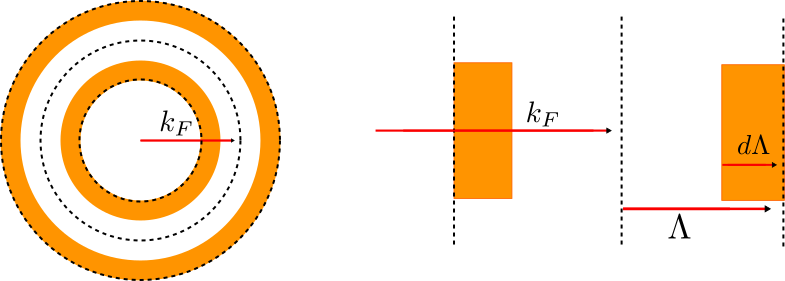
\includegraphics[width=\textwidth]{./figures/fermi-rg.png}
\captionof{figure}{\textbf{Left}: Two directions of integrations for the two-dimensional momentum space. \textbf{Right}: Region of momentum space we are concerned with}
\end{minipage}
\\\\
Since we are only interested in excitations close to the Fermi surface, we can approximate the single particle energy as
\begin{equation}\begin{aligned}
	\xi_\mathbf{K} = \frac{\hbar^2}{2m}\left(K^2 - k_F^2\right) = \frac{\hbar^2}{2m}\left(K - k_F\right)\left(K + k_F\right) \approx \frac{\hbar^2}{2m}\left(K - k_F\right)2k_F = \hbar \left(K-k_F\right)v_F
\end{aligned}\end{equation}
Choosing units such that \(v_F = \hbar = 1\), we get
\begin{equation}\begin{aligned}
	\xi_\mathbf{K} \equiv E_\mathbf{K} - E_F = K - k_F
\end{aligned}\end{equation}
Since we see that \(k_F\) is popping up everywhere, we might as well define \(k = K - k_F\). This will reduce each of the limits by \(k_F\):
\begin{gather}
	\xi_\mathbf{K} = k \\
	S_0 = \int_{-\infty}^\infty d\omega\;\int_0^{2\pi} d\theta \int_{- \Lambda}^{\Lambda}  dk\; \psi_{\mathbf{K},\sigma}^\dagger \psi_{\mathbf{K},\sigma}\label{action}
\end{gather}
\section{Renormalization group calculation}
\subsection*{Noninteracting fixed point}
As mentioned in the previous section, the first step involves reducing the cutoff and integrating out the fast modes. Let the reduced cutoff be \(b\Lambda\), \(b<1\). We can split the action into high momentum and low momentum part:
\begin{equation}\begin{aligned}
	S_0^< &= \int_{-\infty}^\infty d\omega\;\int_0^{2\pi} d\theta \int_{- b\Lambda}^{b\Lambda}dk~\psi_{\mathbf{K},\sigma}^\dagger \left(i\omega - k\right)\psi_{\mathbf{K},\sigma}\\
	S_0^> &= \int_{-\infty}^\infty d\omega\;\int_0^{2\pi} d\theta \int_{\left[-\Lambda,- b\Lambda\right]}^{\left[b\Lambda,\Lambda\right]}dk~\psi_{\mathbf{K},\sigma}^\dagger \left(i\omega - k\right)\psi_{\mathbf{K},\sigma}
\end{aligned}\end{equation}
Then,
\begin{equation}\begin{aligned}
	Z = \int \prod_{k<b\Lambda} d\psi^\dagger_{\mathbf{K},\sigma} d\psi_{\mathbf{K},\sigma} e^{S_0^<}\int \prod_{k>b\Lambda} d\psi^\dagger_{\mathbf{K},\sigma} d\psi_{\mathbf{K},\sigma} e^{S_0^>}
\end{aligned}\end{equation}
Since the modes are decoupled, the result of the high momentum integral does not depend on the low momentum operators; as a result, we can drop that factor that results from the integration. The next step involves rescaling the momenta to recover the original limit. This means we should define new momenta \(k^\prime\):
\begin{equation}\begin{aligned}
k^\prime = b k~.
\end{aligned}\end{equation}
We also need to rescale the energy to recover the limits of the energy integral. Since, in our setup, energy and momentum are dimensionally same, we also define 
\begin{equation}\begin{aligned}
\omega^\prime = b \omega
\end{aligned}\end{equation}
This will modify the action as
\begin{equation}\begin{aligned}
	S_0^< &= \int_{-\infty}^\infty b^{-1} d\omega^\prime\;\int_0^{2\pi} d\theta \int_{-\Lambda}^{\Lambda}b^{-1} dk^\prime\psi_{\mathbf{K},\sigma}^\dagger \left(ib^{-1}\omega^\prime - b^{-1}k^\prime\right)\psi_{\mathbf{K},\sigma}\\
	      &=\int_{-\infty}^\infty d\omega^\prime\;\int_0^{2\pi} d\theta \int_{-\Lambda}^{\Lambda}dk^\prime\psi_{\mathbf{K},\sigma}^\dagger b^{-3} \left(i\omega^\prime - k^\prime\right)\psi_{\mathbf{K},\sigma}
\end{aligned}\end{equation}
Since we are only scaling the radial distance, \(\theta\) will not scale. Since we will compare this new action with the old action eq.~\ref{action}, we need to rescale the fields \(\psi,\psi^\dagger\) to get rid of any global factors. This was the third step mentioned in the previous section. Its obvious that the following rescaling takes care of the \(b^3\) factor: \(\psi^\prime_{\mathbf{K}^\prime} = b^{-\frac{3}{2}}\psi_\mathbf{K}\). The final partition function for the reduced cutoff is
\begin{equation}\begin{aligned}
	Z^< = \int \mathcal{D}{\psi^\prime}^\dagger \mathcal{D}{\psi^\prime}\exp\left\{\int_{-\infty}^\infty d\omega^\prime\;\int_0^{2\pi} d\theta \int_{-\Lambda}^{\Lambda}dk^\prime\psi_{\mathbf K^\prime,\sigma}^\dagger \left(i\omega^\prime - k^\prime\right)\psi_{\mathbf K^\prime,\sigma}\right\}
\end{aligned}\end{equation}
\textbf{This is identical to the partition function we started with. This means that the noninteracting theory is an RG fixed point.}
\subsection{Tree-level quadratic interaction}
We now introduce quadratic interactions through scattering via a potential \(u(k,\omega)\). Owing to momentum conservation, such a term must have the form
\begin{equation}\begin{aligned}
	\int_{-\infty}^\infty d\omega\;\int_0^{2\pi} d\theta \int_{-\Lambda}^{\Lambda}dk \;u({k},\omega)\psi_{\mathbf{K},\sigma}^\dagger\psi_{\mathbf{K},\sigma}
\end{aligned}\end{equation}
Such a term is diagonal in the momentum and we can again carry out the three rescaling operations mentioned previously:
\begin{gather}
k^\prime = b k\\
\omega^\prime = b \omega\\
{\psi^\prime}^\dagger_\mathbf{k^\prime,\sigma}{\psi^\prime}_\mathbf{k^\prime,\sigma} = b^{-3}\psi^\dagger_\mathbf{k,\sigma}\psi_\mathbf{k,\sigma}
\end{gather}
The interaction term then changes to
\begin{equation}\begin{aligned}
\int_{-\infty}^\infty d\omega^\prime\;\int_0^{2\pi} d\theta \int_{-\Lambda}^{\Lambda}dk^\prime \;b u(b{k}^\prime,b\omega^\prime){\psi^\prime_{\mathbf k^\prime}}^\dagger\psi^\prime_{\mathbf k^\prime}
\end{aligned}\end{equation}
We thus see that, as a result of decreasing the cutoff, the interaction potential renormalizes as
\begin{equation}\begin{aligned}
	u({k},\omega) \to b u(b{k},b\omega)
\end{aligned}\end{equation}
To determine the effect of this, we expand \(u\) in a Taylor series around \(\mathbf{k}=0,\omega=0\):
\begin{equation}\begin{aligned}
	u({k},\omega) &= u(0,0) + \omega u_{10} + k u_{01} + \omega^2 u_{20} + k^2 u_{02} + k\omega u_{11} + ...\\
	\to b u(b{k},b\omega) &= bu(0,0) + b b^{-1}\left(\omega^\prime u_{10} + k^\prime u_{01}\right) + b b^{-2} \left({\omega^\prime}^2 u_{20} + {k^\prime}^2 u_{02} + \omega^\prime k^\prime u_{11}\right) + ...\\
			      &= bu(0,0) + \omega^\prime u_{10} + k^\prime u_{01} + b^{-1} \left({\omega^\prime}^2 u_{20} + {k^\prime}^2 u_{02} + \omega^\prime k^\prime u_{11}\right)...
\end{aligned}\end{equation}
where \(u_{mn} = \left(\partial^m_\omega \partial^n_k u\right)_{\omega \to 0, k \to 0}\). The various terms scale as follows:
\begin{equation}\begin{aligned}
	u_{mn} \to b^{1 - m - n}u_{mn}
\end{aligned}\end{equation}
The zeroth order term is relevant - it increases as we scale down to low energies. The first order terms are marginal - they do not change, at least at tree level. Higher terms are irrelevant - they decay upon renormalization.

Even though the zeroth order term is relevant,  such a term already exists in the non-interacting action - the chemical potential term. Since the energies scale as \(\omega^\prime = b\omega\), the chemical potential will also scale as \(\mu^\prime = b \mu\). Hence, we can absorb the relevant zeroth order part of the quadratic fluctuation into the chemical potential:
\begin{gather}
	\mu_\text{eff} = \mu + u(0,0) = b \mu^\prime + bu_{00} = b \mu_\text{eff}^\prime
\end{gather}

The marginal first order terms are also present in the non-interacting action, and hence can again be absorbed into those terms. The conclusion is therefore that adding quadratic interactions do not destroy the non-interacting action, it simply renormalizes certain terms of the non-interacting action.
\subsection{Tree-level quartic interaction}
Next we consider quartic interactions. Translational invariance and time-reversal symmetry requires such scattering events to conserve total momentum and spin:
\begin{equation}\begin{aligned}
\int_{-\infty}^\infty d\omega\;\int_0^{2\pi} d\theta \int_{-\Lambda}^{\Lambda}dk \;V\psi_{\mathbf k_3,\sigma}^\dagger\psi_{\mathbf k_4,\sigma^\prime}\psi_{\mathbf k_1,\sigma}^\dagger\psi_{\mathbf k_2\sigma^\prime} \delta(\mathbf{k_4}+\mathbf{k_3} - \mathbf{k_2} - \mathbf{k_1})\delta({\omega_4}+{\omega_3} - {\omega_2} - {\omega_1})
\end{aligned}\end{equation}
\begin{minipage}{0.45\textwidth}
	Here \(V\) is the scattering potential and in general depends on the momenta and energies. The delta functions conserve total momentum and total energy. Here, \(d\omega\) stands for \(d\omega_1d\omega_2d\omega_3d\omega_4\) and \(dk\) stands for \(dk_1dk_2dk_3dk_4\), Since the potential depends on all the energies and momenta, \(V\) stands for \(V\left(\left\{k_i,\omega_i\right\}\right)\). The fields \(\psi\) of course depend on the momenta and energies. We can easily integrate over \(d\omega_4\) by consuming the energy \(\delta\)-function. Since all the energies can take any value, the condition inside the \(\delta\)-function does not constrain the values of the remaining \(\omega_i\).
\end{minipage}
\hspace*{\fill}
\begin{minipage}{0.45\textwidth}
\begin{center}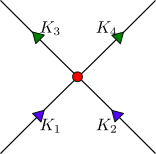
\includegraphics[width=0.85\textwidth]{./figures/term.png}\end{center}
\captionof{figure}{Tree-level four-Fermion scattering}
\end{minipage}\\\\
The result of this integration is
\begin{equation}\begin{aligned}
\int_{-\infty}^\infty d\omega_1 d\omega_2 d\omega_3\;\int_0^{2\pi} d\theta \int_{-\Lambda}^{\Lambda}dk \;V\psi_{\mathbf k_3,\sigma}^\dagger\psi_{\mathbf k_4,\sigma^\prime}\psi_{\mathbf k_1,\sigma}^\dagger\psi_{\mathbf k_2\sigma^\prime} \delta(\mathbf{K_4}+\mathbf{K_3} - \mathbf{K_2} - \mathbf{K_1})
\end{aligned}\end{equation}
where \(\mathbf K_i\) stands for the total momenta and the fields and \(V\) now depend only on the remaining frequencies \(\omega_1,\omega_2,\omega_3\).
 
We now need to tackle the other \(\delta\)-function. Each of the momenta \(\mathbf{k_i}\) can run over the range \([-\Lambda,\Lambda]\). \(k_4 = |\mathbf{K_4}| - k_F\) can take all values satisfying
\begin{equation}\begin{aligned}
k_4 = |\mathbf{K_3} -\mathbf{K_2} - \mathbf{K_1}| - \mathbf{k_F}
\end{aligned}\end{equation}
However, just the momentum conservation equation is not enough to ensure that \(k_4\) is constrained within its allowed range of \(\left[-\Lambda, \Lambda\right]\). For example, if we set \(k_1=-k_F\), \(k_2  = -\Lambda + k_F\) and \(K_3 = \Lambda + k_F\), we get
\begin{equation}\begin{aligned}
k_4 = |K_3 - (K_2 + K_1)| - k_F = |2\Lambda + k_F| - k_F = 2\Lambda
\end{aligned}\end{equation}
which is obviously not allowed. To prevent this, we need to employ a restriction on \(k_4\). The result of the integration without employing the restriction is
\begin{equation}\begin{aligned}
\int_{-\infty}^\infty d\omega_1 d\omega_2 d\omega_3\;\int_0^{2\pi} d\theta \int_{-\Lambda}^{\Lambda}dk_1 dk_2 dk_3 \;V\psi_{\mathbf k_3,\sigma}^\dagger\psi_{\mathbf k_4,\sigma^\prime}\psi_{\mathbf k_1,\sigma}^\dagger\psi_{\mathbf k_2\sigma^\prime}
\end{aligned}\end{equation}
where the \(V\) depends on \(\left\{k_i,\omega_i\right\}, i=1,2,3\). The \(k_4\) in \(\psi_{\mathbf{k_4}}\) stands for \(\mathbf{k_3} -\mathbf{k_2} - \mathbf{k_1}\). Now, in order to employ the above-mentioned restriction, we insert \(\theta(\Lambda - |k_4|)\) inside the integral. That will restrict \(k_4\) to the proper range: \(k_4 \in \left\{-\Lambda,\Lambda\right\}\).
\begin{equation}\begin{aligned}
\int_{-\infty}^\infty d\omega_1 d\omega_2 d\omega_3\;\int_0^{2\pi} d\theta \int_{-\Lambda}^{\Lambda}dk_1 dk_2 dk_3 \;V\psi_{\mathbf k_3,\sigma}^\dagger\psi_{\mathbf k_4,\sigma^\prime}\psi_{\mathbf k_1,\sigma}^\dagger\psi_{\mathbf k_2\sigma^\prime}\theta(\Lambda - |k_4|)
\end{aligned}\end{equation}
We need to check how this Heaviside function \(\theta(\Lambda - |k_4|) = \theta(\Lambda - ||K_3 - K_2 - K_1| - k_F|) \) changes under the scaling. The first step is to change the cutoff from \(\Lambda\) to \(b\Lambda\):
\begin{equation}\begin{aligned}
\theta(\Lambda - |k_4|) \rightarrow \theta(b\Lambda - |k_4|)
\end{aligned}\end{equation}
The next step is to change the integration measure \(dk_i\) to \(dk^\prime_i = \frac{1}{b} dk_i\). This does not modify the Heaviside function but we will just write \(k_4\) in terms of \(k_4^\prime\):
\begin{equation}\begin{aligned}
k_4 &= |K_3 - K_2 - K_1| - k_F \\
      &= b|K_3^\prime - K_2^\prime - K_1^\prime| - k_F\\
      &= b\left(|K_3^\prime - K_2^\prime - K_1^\prime| - \frac{k_F}{b}\right)\\
      &= bk_4^\prime(K_3^\prime , K_2^\prime , K_1^\prime,\frac{k_F}{b})\\
\end{aligned}\end{equation}
\begin{equation}\begin{aligned}
	\implies \theta(b\Lambda - |k_4(k_F)|) = \theta\left(b\Lambda - b\left|k_4^\prime\left(k_F/b\right)\right|\right)
\end{aligned}\end{equation}
Since the condition \(b\Lambda - b|k_4^\prime| > 0\) is the same as \(\Lambda - |k_4^\prime| > 0\), we can write
\begin{equation}\begin{aligned}
\theta(b\Lambda - b|k_4^\prime|) = \theta(\Lambda - |k_4^\prime|)
\end{aligned}\end{equation}
The final step is the rescaling of the fields; this does not affect the Heaviside function in any way. So the total transformation is
\begin{equation}\begin{aligned}
\theta(\Lambda - |k_4(k_F)|) \rightarrow \theta\left(\Lambda - \left|k_4^\prime\left(\frac{k_F}{b}\right)\right|\right)
\end{aligned}\end{equation}
We thus see that the Heaviside function does not return to its original form; in order to remedy this, we replace the Heaviside function by an exponential decay:
\begin{equation}\begin{aligned}
	\exp\left\{-\frac{|k_4|}{\Lambda}\right\}
\end{aligned}\end{equation}
The effect of this exponential decay is similar to the Heaviside function; it suppresses the effect of the \(k_4\) that lie outside the allowed region,  \(|k_4| > \Lambda\). In the limit of \(b \rightarrow 0\), we will have \(\Lambda \rightarrow 0\), and the exponential will then take the form
\begin{equation}\begin{aligned}
	\lim_{\Lambda \to 0} \exp\left\{-\frac{|k_4|}{\Lambda}\right\} = \begin{cases} 1, &\text{ when } |k_4|<\Lambda \\ 0, &\text{ when } |k_4|>\Lambda \end{cases} = \theta(\Lambda - |k_4|)
\end{aligned}\end{equation}
In the limit of very low energy, we recover the Heaviside function behavior. The quartic term takes the form
\begin{equation}\begin{aligned}
	\int_{-\infty}^\infty d\omega_1 d\omega_2 d\omega_3\;\int_0^{2\pi} d\theta \int_{-\Lambda}^{\Lambda}dk_1 dk_2 dk_3 \;V\psi_{\mathbf k_3,\sigma}^\dagger\psi_{\mathbf k_4,\sigma^\prime}\psi_{\mathbf k_1,\sigma}^\dagger\psi_{\mathbf k_2\sigma^\prime}\exp\left\{-\frac{|k_4|}{\Lambda}\right\}
\end{aligned}\end{equation}
To see how this exponential factor scales with the renormalization, note that
\begin{equation}\begin{aligned}
\label{k4}
k_4 &= \left|\mathbf{K_3} - \mathbf{K_2} - \mathbf{K_1}\right| - k_F \\
    &= \left|\left(k_3 + k_F\right)\hat k_3 - \left(k_2 + k_F\right)\hat k_2 - \left(k_1 + k_F\right)\hat k_1\right| - k_F\\
    &=\left|k_F\left(\hat k_3 - \hat k_2 - \hat k_1\right) + \left(\mathbf{k_3} - \mathbf{k_2} - \mathbf{k_1}\right)\right| - k_F
\end{aligned}\end{equation}
The second term, \(\mathbf{k_3} - \mathbf{k_2} - \mathbf{k_1}\), is typically of order at most \(\Lambda\), because that is the highest value that the momenta can take. Therefore, the only situation in which this second term can be comparable to the first term (of order \(k_F\)) is when
\begin{equation}\begin{aligned}
k \sim \Lambda \sim k_F
\end{aligned}\end{equation}
Then, \(k_4\) will also be of the same order: \(k_4 \sim \Lambda \sim k_F\). However, from the exponential decay, we know that the only \(k_4\) that can survive are the ones in the range \(k_4 \ll \Lambda\). Therefore, we can neglect the second term in eq.~\ref{k4}, and take
\begin{equation}\begin{aligned}
	k_4 \approx k_F\left|\left(\hat k_3 - \hat k_2 - \hat k_1\right)\right| - k_F
\end{aligned}\end{equation}
Under the renormalization, the unit vectors will not scale because they are simply directions on the Fermi surface and are dimensionless. Therefore,
\begin{equation}\begin{aligned}
	\exp\left\{-\frac{\left|\left|k_F\left(\hat k_3 - \hat k_2 - \hat k_1\right)\right| - k_F\right|}{\Lambda}\right\}&\rightarrow\exp\left\{-\frac{\left|\left|k_F\left(\hat k_3 - \hat k_2 - \hat k_1\right)\right| - k_F\right|}{b\Lambda}\right\}\\
															 &=\exp\left\{-\frac{\left|\left|k_F\left(\hat k_3 - \hat k_2 - \hat k_1\right)\right| - k_F\right|}{\Lambda}\left(1 + \frac{b-1}{b}\right)\right\}\\
	\implies \exp\left\{-\frac{|k_4|}{\Lambda}\right\} &\rightarrow \exp\left\{-\frac{|k_4|}{\Lambda}\right\}\exp\left\{\left(1 - \frac{1}{b}\right)\frac{|k_4|}{\Lambda}\right\}
\end{aligned}\end{equation}
Therefore, under the renormalization, the exponential gets multiplied by a factor
\begin{equation}\begin{aligned}
	\exp\left\{\left(1 - \frac{1}{b}\right)\frac{|k_4|}{\Lambda}\right\}
\end{aligned}\end{equation}
As \(b \rightarrow 0\), the argument of the exponential will go to \(-\infty\) and the factor will vanish. The only way to make this term survive is by making the argument of the exponential vanish. This will happen if \(|k_4|\) vanishes:
\begin{gather}
	|k_4| \approx k_F\left(\left|\left(\hat k_3 - \hat k_2 - \hat k_1\right)\right| - 1\right)=0\\
		\implies \left|\left(\hat k_3 - \hat k_2 - \hat k_1\right)\right| = 1\\
		\implies \left(\hat k_3 - \hat k_2 - \hat k_1\right)^2 = 1\label{eqtn}
\end{gather}
\begin{minipage}{300pt}
	The only momenta that will survive are the ones in the directions that satisfy the above equation. To find the possible angles for that equation, let \(\hat x \equiv \hat k_3\) and \(\hat k_{1,2} = \cos \theta_{1,2}\hat x + \sin\theta_{1,2}\hat y\). As defined, \(\theta_1\) is the angle between \(\hat k_1\) and \(\hat k_3\), and \(\theta_2\) is that between \(\hat k_2\) and \(\hat k_3\). 
\end{minipage}
\begin{minipage}{200pt}
	\begin{center}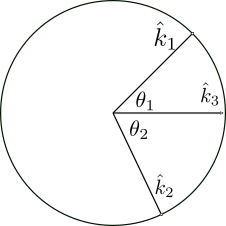
\includegraphics[scale=0.2]{./figures/term2.png}\end{center}
	\captionof{figure}{Three remaining momenta and angles between them}
\end{minipage}\\
Substituting this in eq.~\ref{eqtn} gives
\begin{gather}
 1 + \cos\theta_1\cos\theta_2 + \sin\theta_1\sin\theta_2= \cos\theta_1 + \cos\theta_2\\
 \implies  1 + \cos\left(\theta_1 - \theta_2\right) = \cos\theta_1 + \cos\theta_2\\
\implies  2\cos^2\frac{\theta_1 - \theta_2}{2} = 2\cos\frac{\theta_1 + \theta_2}{2}\cos\frac{\theta_1 - \theta_2}{2}\\
\implies  \cos\frac{\theta_1 - \theta_2}{2}\left(\cos\frac{\theta_1 - \theta_2}{2} - \cos\frac{\theta_1 + \theta_2}{2}\right) =0
\end{gather}
The solutions of this equation are
\begin{equation}\begin{aligned}
	\theta_1 - \theta_2 = \pm \pi \text{ and } \theta_1 - \theta_2 = \pm\left(\theta_1 + \theta_2\right)
\end{aligned}\end{equation}
Take the first solution. It gives \(\theta_1 = \theta_2 \pm \pi\), which in turn means
\begin{equation}\begin{aligned}
\label{cos}
\cos \theta_1 = \cos \left(\pi \pm \theta_2\right) = -\cos \theta_2
\end{aligned}\end{equation}
and
\begin{equation}\begin{aligned}
\label{sin}
\sin \theta_1 = \pm \sin\left(\pi \pm \theta_2\right) = \pm \times \mp \sin\theta_2 = -\sin\theta_2
\end{aligned}\end{equation}
Combining eqs.~\ref{cos} and \ref{sin}, we get
\begin{equation}\begin{aligned}
\hat k_1 = - \hat k_2
\end{aligned}\end{equation}
The second solutions gives \(\theta_1 = \theta_2 \pm \left(\theta_1 + \theta_2\right)\). The two possibilities are
\begin{equation}\begin{aligned}
\theta_1 = 0
\end{aligned}\end{equation}
and
\begin{equation}\begin{aligned}
\theta_2 = 0
\end{aligned}\end{equation}
Since \(\theta_{1,2}\) is the angle made by \(\hat k_{1,2}\) against \(\hat k_3\), the two solutions simply mean
\begin{equation}\begin{aligned}
\hat k_1 = \hat k_3
\end{aligned}\end{equation}
and
\begin{equation}\begin{aligned}
\hat k_2 = \hat k_3
\end{aligned}\end{equation}

The three cases where the momenta might survive are
\begin{itemize}
	\item \(\hat k_1 = - \hat k_2\)\\
	\item \(\hat k_1 = \hat k_3\)\\
	\item \(\hat k_2 = \hat k_3\)
\end{itemize}
We can now consider the scaling of \(V(\left\{\mathbf{k_i},\omega_i\right\}) (= V\left(\left\{k_i,\omega_i,\theta_i\right\}\right))\) for these three cases only. Under the process of scaling,
\begin{equation}\begin{aligned}
d\omega_1 d\omega_2 d\omega_3 &\rightarrow b^{3}d\omega^\prime_1 d\omega^\prime_2 d\omega^\prime_3\\
dk_1 dk_2 dk_3 &\rightarrow b^{3}dk^\prime_1 dk^\prime_2 dk^\prime_3\\
\psi_{\mathbf k_3,\sigma}^\dagger\psi_{\mathbf k_4,\sigma^\prime}\psi_{\mathbf k_1,\sigma}^\dagger\psi_{\mathbf k_2\sigma^\prime} &\rightarrow b^{-3}{\psi^\prime}_{\mathbf k_3,\sigma}^\dagger{\psi^\prime}_{\mathbf k_4,\sigma^\prime}{\psi^\prime}_{\mathbf k_1,\sigma}^\dagger{\psi^\prime}_{\mathbf k_2\sigma^\prime}
\end{aligned}\end{equation}
The net change is thus no scaling, because the \(b^6\) from scaling of \(dk\) and \(d\omega\) cancels the scaling of the fields. Thus, the potential transforms trivially:
\begin{equation}\begin{aligned}
	V(\left\{k_i,\omega_i,\theta_i\right\}) \rightarrow V(\left\{k_i,\omega_i,\theta_i\right\}) = V(\left\{b k_i^\prime,b \omega_i^\prime,\theta_i\right\})
\end{aligned}\end{equation}
Similar to the quadratic case, we expand the potential around \(k=0,\omega=0\).
\begin{equation}\begin{aligned}
V = V(0,0,\theta) + k \partial_k V(0,0,\theta) + \omega \partial_\omega V(0,0,\theta) + O(2)
\end{aligned}\end{equation}
The zeroth order term scales marginally:
\begin{equation}\begin{aligned}
V(0,0,\theta) \rightarrow V(0,0,\theta)
\end{aligned}\end{equation}
The first order terms scale irrelevantly:
\begin{equation}\begin{aligned}
k \partial_k V(0,0,\theta) = bk \partial_k V(0,0,\theta)
\end{aligned}\end{equation}
Higher terms will scale more irrelevantly. From this analysis, we can say that we might as well set \(k=0\) and \(\omega=0\) because the dependence on momenta and frequency does not produce any scaling higher than irrelevance, and keep only the \(\theta\) dependence. In other words, we will consider the dependence of \(V\) on \(\theta\) only at the Fermi surface (where \(k=\omega=0\)), because dropping the momenta and frequency dependence does not lose any relevance or marginally.
 
For cases where \(\Lambda\) has been shrunk down to a small value (such as the case we are considering- exactly on the Fermi surface), the four momenta \(\mathbf{k_1}\) through \(\mathbf{k_4}\) must lie on the thin ring, and they will more or less have the same values, say \(k\). Then, the momentum conservation condition gives \(\hat k_1 + \hat k_2 = \hat k_3 + \hat k_4\). Using the three possible cases along with this momentum conservation equation then gives
\begin{itemize}
	\item \(\hat k_1 = - \hat k_2\) \text{ and } \(\hat k_3 = - \hat k_4\)\\
	\item \(\hat k_1 = \hat k_3\) \text{ and } \(\hat k_2 = \hat k_4\)\\
	\item \(\hat k_2 = \hat k_3\) \text{ and } \(\hat k_1 = \hat k_4\)
\end{itemize}
The last two cases are essentially same; together they imply that the incoming momenta match the outgoing momenta. The two separate cases can be obtained simply by permuting the particles in the potential function. Since the outgoing momenta are individually equal to the incoming momenta, the potential will depend only on the incoming momenta; the outgoing momenta are fixed automatically by the incoming momenta. 
\begin{equation}\begin{aligned}
	V(\left\{\theta_i\right\}) = V_1(\theta_1,\theta_2)
\end{aligned}\end{equation}
From rotational symmetry, we know that \(V_1(\theta_1,\theta_2) = V_1(\theta_1 - \theta_2,0) \equiv V_1(\theta_1 - \theta_2)\). The conclusion is that for the last two cases, the potential function takes the form
\begin{equation}\begin{aligned}
V_1(\theta_1 - \theta_2)
\end{aligned}\end{equation}
on the Fermi surface. For the first case, we have 
\begin{equation}\begin{aligned}
	V(\left\{\theta_i\right\}) = V_2(\theta_1,-\theta_1,\theta_3,-\theta_3) = V_2(\theta_1 - \theta_3)
\end{aligned}\end{equation}
Summarizing, \textbf{for the two cases in which the momenta can survive on the Fermi surface, we get two marginal couplings.} They are marginal because they are independent of the momenta and frequency. The two couplings are \(V_1(\theta_1 - \theta_2)\) for the case when the incoming momenta equal the outgoing momenta, and \(V_2(\theta_1 - \theta_3)\) for the case when the net incoming momentum as well the net outgoing momentum are 0.
\subsection{1-loop renormalization for \(\mathbf{V_1}\)}
\begin{minipage}{350pt}

	We next consider interactions that involve virtual particles. Consider first the function \(V_1\), for which \(k_1=k_3\). Let the four particles be labeled \(1,2,3\) and 4. Since the scatterings will be caused by virtual particles, one such way of producing such a scattering is when particle 1 scatters into particle 3 by absorbing and releasing a virtual particle. Since we have set \(k_i = 0\) and \(\omega_i = 0\), the virtual particles should not provide any net energy or momentum, hence both the incoming and outgoing virtual particles will carry same energy and momentum. The curved lines represent the virtual particles.
\end{minipage}
\begin{minipage}{200pt}
	\begin{center} 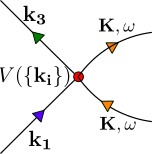
\includegraphics[scale=0.35]{./figures/term1.png}\end{center}
	\captionof{figure}{One half a one-loop four-Fermion scattering}
\end{minipage}\\\\
There will be a similar scattering between the second and fourth particles. They will absorb and emit the virtual particles emitted by the previous scattering. The total process is shown below. Since we want to calculate the differential contribution of this process to the potential, \(dV_1\), we will restrict the momenta to a small part of the bandwidth \(\left[\Lambda - d\Lambda, \Lambda\right]\). The virtual particles will thus have momenta \(\mathbf{K}\) close to the bandwidth: \(|K - k_F|\sim \Lambda\). Also, since there is no energy transfer required (\(k_1=k_3\)), both the virtual particles will have the same energy \(\omega\). This means they will have identical propagators:
\begin{equation}\begin{aligned}
G(\omega,\mathbf{K}) = \frac{1}{i\omega - E(\mathbf{K})}
\end{aligned}\end{equation}
The contribution to \(dV_1\) from such a scattering is thus of the form
\begin{equation}\begin{aligned}
\int d(\theta_1 - \theta_2) \int_{-\infty}^\infty d\omega \int_{d\Lambda}dK V_1(\theta_1 - \theta_2) G^2(\mathbf{K},\omega)
\end{aligned}\end{equation}
This integral will vanish for the following reason. The complex function \(G^2 = \left(i\omega - E\right)^{-2}\) has just one pole at \(i\omega = E\). This pole lies in one particular half of the complex plane. To perform the integration, we can just close the contour in the other half of the complex plane. This plane will have no poles and this integral will evaluate to zero.
\begin{center}
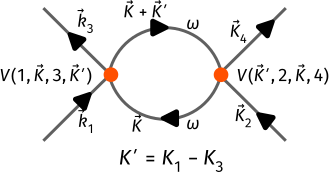
\includegraphics[scale=0.3]{./figures/term3.png}
\captionof{figure}{Complete diagram for scattering with virtual particles}
\end{center}
That this vanishes is due to the fact that both the Greens functions are identical. This would not have been the case if, say, one of the virtual particles was a hole of frequency \(\omega\) and momentum \(-K\). Itss energy would then have been \(-\omega\) and the propagator would have been
\begin{equation}\begin{aligned}
\tilde G(\omega,\mathbf{-K}) = \frac{1}{-i\omega - E(\mathbf{-K})}
\end{aligned}\end{equation}
The complex function inside the integral would then have been
\begin{equation}\begin{aligned}
\label{prop}
G(\omega,\mathbf{K})\tilde G(\omega,\mathbf{-K}) = \frac{1}{i\omega - E(\mathbf{K})}\frac{1}{-i\omega - E(\mathbf{-K})}
\end{aligned}\end{equation}
This will have poles in both the upper and lower halves and would have given non-zero contribution. However, as it stands, there is no momentum change between the two virtual particles, so we cannot go from a particle at \(K \sim k_F + \Lambda\) to a hole at \(K \sim k_F - \Lambda\) and hence both the virtual particles will either be holes or particles. Such a switch from particle to hole would require a momentum transfer of order \(\sim \Lambda\).
Another way of causing such a scattering would be by replacing \(1 \leftrightarrow 2\). The difference then would be that since particle 1 will be scattering into particle 4 and since they do not have the same momenta, these virtual particles will now carry different momenta, effectively causing a net change in momenta. More specifically, we will allow one of these virtual particles to have a momentum \(\mathbf{K}\) and the other to have a momentum \(\mathbf{K+Q}\). This will produce a net momentum transfer of \(\mathbf{Q}\).
\begin{center}
\includegraphics[scale=0.3]{./figures/term4.png}
\captionof{figure}{Second four-Fermion scattering - momenta interchanged}
\end{center}
For small momentum transfer \(Q \ll \Lambda\), the two poles will again be on the same half of the complex plane and we will again get zero. For a large \(Q \sim k_F\), things are different though. Such a momentum transfer can now connect particles with holes. However, note that since both the momenta \(\mathbf{K}\) and \(\mathbf{K}+\mathbf{Q}\) must lie on the shells of width \(d\Lambda\) around the bandwidth, a large value of \(Q\) will severely constrain the angles at which \(\mathbf{K}\) can lie. To find the available region for \(\mathbf{K}\), let the angle between \(\mathbf{K}\) and \(\mathbf{Q}\) be \(\alpha\). Also, let \(\mathbf{K}+\mathbf{Q}\equiv\mathbf{K}^\prime\). Both \(\mathbf{K}\) and \(\mathbf{K}^\prime\) are of order \(\Lambda \pm d\Lambda\), while \(\mathbf{Q}\)  is of order \(k_F\). From the cosine law of triangles, we can write

\begin{minipage}{280pt}
\begin{gather}
\mathbf{K}+\mathbf{Q}|^2 = |\mathbf{K}^\prime|^2\\
\implies K^2 + Q^2 + 2KQ\cos \alpha = {K^\prime}^2\\
\implies \cos \alpha = \frac{{K^\prime}^2 - K^2 - Q^2}{2KQ}
\end{gather}
Since \(K \sim K^\prime\), we can write \({K^\prime}^2 - K^2 \approx 2K^\prime \left(K^\prime - K\right)\). Therefore,
\begin{equation}\begin{aligned}
	\cos \alpha \approx \frac{2K^\prime\left(K^\prime - K\right) - Q^2}{2K^\prime Q} = \frac{K^\prime - K}{Q} - \frac{Q}{2K^\prime}
\end{aligned}\end{equation}
\end{minipage}
\begin{minipage}{250pt}
	\begin{center}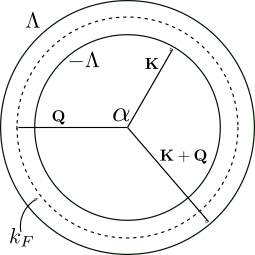
\includegraphics[scale=0.28]{./figures/term5.png}\end{center}
	\captionof{figure}{Finding available region for \(\mathbf{K}\)}
\end{minipage}
 
The second term is typically of the order \(-\frac{k_F}{2\Lambda}\) and does not change. The term that will change is the one that involves \(K^\prime - K\). The maximum value of \(K^\prime - K\) is \\\(\Lambda + d\Lambda  - \left(-\Lambda - d\Lambda\right) = 2\left(\Lambda+d\Lambda\right)\), while the minimum is
\(2\left(\Lambda-d\Lambda\right)\). Therefore, the wiggle-room for \(\alpha\) is
\begin{equation}\begin{aligned}
d\cos \alpha = \frac{4 d\Lambda}{k_F}
\end{aligned}\end{equation}
Since \(\sin \alpha\) is of order unity, we can write
\begin{equation}\begin{aligned}
d\alpha \sim \frac{d\Lambda}{K_F}
\end{aligned}\end{equation}
Therefore, the total region over which the momenta can move is
\begin{equation}\begin{aligned}
\int d\theta \int dk \sim \frac{d\Lambda}{k_F}d\Lambda = \frac{d\Lambda^2}{k_F}
\end{aligned}\end{equation}
Therefore, the total contribution to \(V_1\) from this scattering is
\begin{equation}\begin{aligned}
	d V_1 \sim d\Lambda^2 \implies \lim_{d\Lambda \to 0} \frac{\mathrm{d}V_1}{\mathrm{d}\Lambda} = \lim_{d\Lambda \to 0} d\Lambda = 0
\end{aligned}\end{equation}
\begin{minipage}{280pt}
	The final scattering process that we can consider is when the two incoming particles 1 and 2 scatter to produce two virtual particles which then annihilate to produce the two outgoing particles. Since we have placed both the incoming particles on the Fermi surface, they have total (as well as individual) energy zero, so the two virtual particles produced must have equal and opposite energies \(\pm \omega\). We can however allow a momentum transfer of \(\mathbf{Q}\), as in the previous process. The two momenta will then be \(\mathbf{K}\) and \(\mathbf{Q} -\mathbf{K}\).
 
Note that the same considerations of angle wiggle room will apply here. Both \(\mathbf{K}\) and \(\mathbf{Q-K}\) have to lie on the thin shells of width \(d\Lambda\) at \(\pm \Lambda\). Since \(\mathbf{Q}\) is typically large, this will again constrain the angle \(\alpha\) that can be subtended by the momentum \(\mathbf{K}\). We again get a contribution of \(\frac{d\Lambda^2}{k_F}\) from the \(\theta\) and \(K\) integrals, meaning this diagram will also not contribute anything.\\
\end{minipage}
\hspace*{20pt}
\begin{minipage}{250pt}
	\begin{center}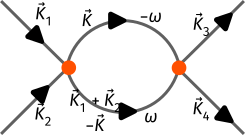
\includegraphics[scale=0.3]{./figures/term6.png}\captionof{figure}{Third diagram of \(V_1\). Incoming particles scatter into virtual ones.}\label{bcs1}\end{center}
\end{minipage}
 
\textbf{The conclusion is that there is no renormalization of the first function \(V_1\) at one loop level.}
\subsection{1-loop renormalization for \(\mathbf{V_2}\)}
We next consider the renormalization of the second function \(V_2\), for which the condition is that the total incoming and outgoing momenta are zero (\(k_1 + k_2 = k_3 + k_4 = 0\)), although the individual values can be non-zero. Similar to the first diagram for \(V_1\), we will have a process where the particles 1 and 3 scatter by emitting and absorbing virtual particles. The difference, however, is that unlike the \(V_1\) diagram where the particles 1 and 3 had same momenta and hence the virtual particles were unable to carry away any net momenta, here the particles 1 and 3 have different momenta and the virtual particles are allowed to carry a net momenta \(\mathbf{Q}\). So the virtual particles will carry momenta \(\mathbf{K}\) and \(\mathbf{Q-K}\). The energies are still zero because we are the Fermi surface, so the virtual particles will carry the same frequency \(\omega\). 
\begin{center}
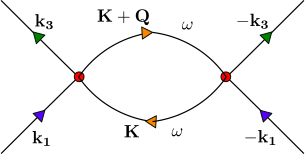
\includegraphics[scale=0.3]{./figures/term7.png}
\captionof{figure}{First diagram for \(V_2\). Particles 1 and 3 scatter via virtual particles}
\label{bcs2}
\end{center}
This diagram will give zero for the same reasons as above: If \(\mathbf{Q}\) is sufficiently small, it will not be able to connect particle and hole virtual states, so the poles in the Green's function will be on the same half and we will close the contour on the other half. If the transfer momentum is sufficiently large so as to connect holes and particles, it will severely constrain the angular width of \(\mathbf{K}\), and the contribution will go as \(d\Lambda^2\), as shown above.
 
\begin{minipage}{280pt}
	The second diagram for \(V_2\) is obtained simply by interchanging the particles 3 and 4 in fig.~\ref{bcs2}. This will also vanish by the same argument. The third diagram is obtained by allowing the particles 1 and 2 to scatter into two virtual particles. Since the total momentum and energy of the incoming particles is zero, these virtual particles will have momenta and energy \(\pm \mathbf{K}\) and \(\pm \omega\) respectively. This diagram is topologically similar to the third diagram for the \(V_1\) function, fig.~\ref{bcs1}. The difference however is that in this diagram, \(Q=0\). This means the angular width will not be constricted, and the vector \(\mathbf{K}\) can roam freely over the entire shell. This is the only one-loop diagram that vanish; it neither has a very large momentum to reduce the contribution to \(d\Lambda^2\),nor does it have poles on the same half- one of the particles is a hole, with energy and momentum \(-\omega,-\mathbf{K}\).
\end{minipage}
\hspace*{20pt}
\begin{minipage}{250pt}
\begin{center}
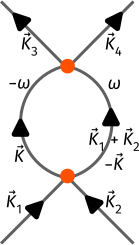
\includegraphics[scale=0.3]{./figures/term8.png}
\captionof{figure}{First diagram for \(V_2\). Particles 1 and 3 scatter via virtual particles}
\label{bcs3}
\end{center}
\end{minipage}
 
The contribution to \(V_2\) from this diagram is obtained as follows. The first scattering has a potential term of the form \(V_2(\theta_1 - \theta_3)\). Here \(\theta_1\) is the angle for the incoming particle, and \(\theta_3\) is that of the virtual particle, which we are integrating by the dummy index \(\theta\), so the potential term becomes \(V_2(\theta_1 - \theta)\). Next comes propagators for the particle and hole. This will be exactly of the form mentioned in eq.~\ref{prop}. The final term is another potential term for the second scattering. Here the first scatterer is a virtual particle so we replace \(\theta_1\) with \(\theta\) and the third scatterer is the outgoing particle with angle \(\theta_3\). This term is \(V_2(\theta - \theta_3)\). The total contribution to \(V_2\) is
\begin{equation}\begin{aligned}
dV_2(\theta_1 - \theta_3) = -\frac{1}{2}\int_0^{2\pi} \frac{d\theta}{2\pi} \int_{d\Lambda}\frac{dk}{2\pi} \int_{-\infty}^\infty \frac{d\omega}{2\pi} V_2(\theta_1 - \theta) G(\omega,\mathbf{K})\tilde G(\omega,\mathbf{-K}) V_2(\theta - \theta_3)
\end{aligned}\end{equation}
The factor of half in front comes from the \(2!\) in Dyson's expansion. The minus sign comes from the exchange of operations of creation and annihilation. The Greens function by default has a destruction followed by creation, but since this process has two consecutive creation, we need to interchange an operator which brings the minus sign. Since the potential terms do not depend on the energy and momentum, this integration simplifies to
\begin{equation}\begin{aligned}
dV_2(\theta_1 - \theta_3) = -\frac{1}{16\pi^3}\int_0^{2\pi} d\theta V_2(\theta_1 - \theta)V_2(\theta - \theta_3)\int_{d\Lambda}dk \int_{-\infty}^\infty d\omega  \frac{1}{i\omega - E(\mathbf{K})}\frac{1}{-i\omega - E(\mathbf{-K})}
\end{aligned}\end{equation}
The first order of business is to do the energy integral. Since \(E(k) = E(-K)\), the two poles are  \(i\omega = \pm E(k)\). We will close the contour in the upper half. The result of the integration is
\begin{equation}\begin{aligned}
\int_{-\infty}^\infty d\omega  \frac{1}{i\omega - E(\mathbf{K})}\frac{1}{-i\omega - E(\mathbf{K})} &= \int_{-\infty}^\infty d\omega  \frac{1}{\omega^2 + E^2}\\
											       &=2 \int_0^\infty d\omega  \frac{1}{\omega^2 + E^2}\\
											       &= 2\frac{1}{E} \arctan (\omega) \bigg\vert_0^\infty\\
											       &= \frac{\pi}{E(K)}
\end{aligned}\end{equation}
The momentum integral can now be performed:
\begin{equation}\begin{aligned}
	\int_{d\Lambda} dk \frac{1}{E(K)} &= \left(\int_{-\Lambda-d\Lambda}^{-\Lambda} + \int_{\Lambda}^{\Lambda+d\Lambda}\right)\frac{dk}{E(K)}\\
				&= 2\int_{\Lambda}^{\Lambda+d\Lambda}\frac{dk}{E(K)}\\
				&=2\left[\frac{1}{\Lambda + d\Lambda} - \frac{1}{\Lambda}\right]\\
				&=2\frac{-d\Lambda}{\Lambda}\\
\end{aligned}\end{equation}
Putting these two integrations into the expression for \(dV_2\) gives
\begin{equation}\begin{aligned}
dV_2 &= \frac{1}{8\pi^2}\frac{d\Lambda}{\Lambda}\int_0^{2\pi} d\theta V_2(\theta_1 - \theta)V_2(\theta - \theta_3)\\
\implies \Lambda\frac{\mathrm{d}V_2}{\mathrm{d}\Lambda} &= \frac{1}{8\pi^2}\int_0^{2\pi} d\theta V_2(\theta_1 - \theta)V_2(\theta - \theta_3)
\end{aligned}\end{equation}
To solve this equation, note that since \(V_2\) depends only on the angular variable \(\theta\), it can be expanded in a series of \(e^{im\theta}\), because the exponentials form a complete set:
\begin{equation}\begin{aligned}
	V_2(\theta_1 - \theta_3) = \sum_m \tilde V_{2,m} e^{im\left(\theta_1 - \theta_3\right)}
\end{aligned}\end{equation}
Similarly expanding the other \(V_2\) and substituting them in the coupling equation gives
\begin{equation}\begin{aligned}
	\Lambda \sum_m \frac{\mathrm{d}\tilde V_{2,m}}{\mathrm{d}\Lambda} e^{im\left(\theta_1 - \theta_3\right)} &= \frac{1}{8\pi^2}\int_0^{2\pi} d\theta \sum_{m_1,m_3}\tilde V_{2,m_1}\tilde V_{2,m_3}e^{i\left(m_1\theta_1 - m_3\theta_3\right)}e^{i\theta\left(m_3 - m_1\right)}\\
											   &=\frac{1}{8\pi^2}\sum_{m_1,m_3}\tilde V_{2,m_1}\tilde V_{2,m_3}e^{i\left(m_1\theta_1 - m_3\theta_3\right)}2\pi \delta\left(m_3 - m_1\right)\\
											   &=\frac{1}{4\pi}\sum_{m}\tilde V_{2,m}^2e^{im\left(\theta_1 - \theta_3\right)}\\
\end{aligned}\end{equation}
Since the \(\exp\left\{im\left(\theta_1 - \theta_3\right)\right\}\) form a linearly independent set, we can compare the coefficients directly and write down
\begin{equation}\begin{aligned}
\label{rgeq}
\Lambda \frac{\mathrm{d}\tilde V_{2,m}}{\mathrm{d}\Lambda} &=\frac{1}{4\pi}\tilde V^2_{2,m} \\
\implies \frac{\mathrm{d}\tilde V_{2,m}}{\mathrm{d}\Lambda} &=\frac{1}{4\pi \Lambda}\tilde V^2_{2,m}
\end{aligned}\end{equation}
We can integrate this equation easily:
\begin{gather}
\int_{\tilde V_{2,m}(\Lambda_0)}^{\tilde V_{2,m}(\Lambda)} \frac{d\tilde V_{2,m}}{\tilde V^2_{2,m}} =\frac{1}{4\pi}\int_{\Lambda_0}^\Lambda \frac{d\Lambda}{\Lambda}\\
\implies \frac{1}{\tilde V_{2,m}(\Lambda_0)} - \frac{1}{\tilde V_{2,m}(\Lambda)} = \frac{1}{4\pi}\ln \frac{\Lambda}{\Lambda_0}\\
\implies \tilde V_2(\Lambda) = \tilde V_2(\Lambda_0)\left(1 + \frac{\tilde V_2(\Lambda_0)}{4\pi}\ln \frac{\Lambda_0}{\Lambda}\right)^{-1}
\end{gather}
In the last step I dropped the \(m\) to simplify the notation. This is the expression that describes the behavior of the function \(V_2\) as we decrease the bandwidth.
 
From the RG equation eq.~\ref{rgeq}, we can draw the following conclusions:
\begin{itemize}
	\item Since the RHS is always positive, \(\tilde V_{2,m}\) will always decrease when we reduce the bandwidth and come  down to low energies.
	\item There are two fixed points under the RG flow: One is at \(\tilde V_{2,m} = 0\) because there the rate of change becomes zero. The other is at \(\tilde V_{2,m} = -\infty\) because if the coupling reaches that value, it will remain at that value.
	\item \textbf{If a function \(\tilde V_{2,m}\) is initially positive (repulsive in nature), it will, as mentioned in the first point, shrink under the RG and decay to zero.
	\item If \(\tilde V_{2,m}\) is initially negative (attractive in nature), it will decrease to increasingly negative values until it reaches \(-\infty\).}
\end{itemize}
\section{Conclusions}
\subsection{Landau's theory of Fermi liquids}
For the time being, let us ignore the \(V_2\) terms and pretend we have only the \(V_1\) terms. At very low energies, we then have just the noninteracting terms and the \(V_1(\theta_1 - \theta_2)\) terms. Using them, we can write a low energy effective Hamiltonian for the system. The noninteracting part is the same
\begin{equation}\begin{aligned}
\mathcal{H}_0 = \sum_{\theta}\epsilon_\theta \hat n_{\theta}
\end{aligned}\end{equation}
\(\epsilon_\theta\) is the renormalized kinetic energy of the excitations at the Fermi surface, having a momentum \(\mathbf{K}=k_F\left(\cos \theta \hat x + \sin \theta \hat y\right)\). The sum over \(\theta\) is just the sum over the Fermi surface; the momenta on the Fermi surface are parametrised by just one variable, the angular coordinate \(\theta\). The only other term that is not irrelevant after the RG is the four-Fermion interaction term: 
\begin{equation}\begin{aligned}
\sum_{\theta_1\theta_2\theta_4\theta_4}V_1(\theta_1,\theta_2,\theta_3,\theta_4)c^\dagger_{\theta_4} c^\dagger_{\theta_3}c_{\theta_2}c_{\theta_1}
\end{aligned}\end{equation}
But since \(V_1\) is only non-irrelevant on the condition \(\theta_4 = \theta_2, \theta_3=\theta_1\), this term simplifies to
\begin{equation}\begin{aligned}
\sum_{\theta_1\theta_2}V_1(\theta_1-\theta_2)c^\dagger_{\theta_2} c^\dagger_{\theta_1}c_{\theta_2}c_{\theta_1} = \sum_{\theta_1\theta_2}V_1(\theta_1-\theta_2) \hat n_{\theta_2} \hat n_{\theta_1}
\end{aligned}\end{equation}
Combining this with the free Hamiltonian \(\mathcal{H}_0\) gives
\begin{equation}\begin{aligned}
\mathcal{H}_\text{FL} = \sum_{\theta}\epsilon_\theta \hat n_{\theta} + \sum_{\theta_1\theta_2}V_1(\theta_1-\theta_2) \hat n_{\theta_2} \hat n_{\theta_1}
\end{aligned}\end{equation}
\textbf{This is essentially the Hamiltonian obtained from Landau's Fermi liquid theory under the assumption of \textit{adiabatic continuity}}. The first term is the renormalized single-particle kinetic energy of the low energy excitations, while the second term is the number-diagonal interaction between these excitations. The assumption of \textit{adiabatic continuity} was invoked when we ignored the presence of the \(V_2\) terms and hence avoided any phase transitions. This also justifies why Landau did not need to keep higher order diagonal terms In the Hamiltonian- such terms are irrelevant.
 
\begin{minipage}{300pt}
The number operators here correspond to the renormalized ones. At tree level, the only diagram corresponding to this is fig.~\ref{susc1}. It represents the noninteracting susceptibility of the Fermi gas. Its simple to write down the two Green's functions and compute the contribution of this diagram:
\begin{equation}\begin{aligned}
\chi_0(q) = \int d\omega \frac{1}{i\omega - E(q)}\frac{1}{-i\omega  -E(-q)}
\end{aligned}\end{equation}
\end{minipage}
\hspace*{30pt}
\begin{minipage}{200pt}
\begin{center}
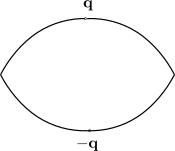
\includegraphics[scale=0.3]{./figures/term10.png}
\captionof{figure}{Noninteracting susceptibility for Fermi liquid}
\label{susc2}
\end{center}
\end{minipage}
 
Note that since we are very close to the Fermi surface, even a very small \(q\) can connect particle and hole states.We do not need to bother with the integral. Higher order diagrams consisting of one and more loops are shown in fig.~\ref{susc2}. The term in the bracket is a geometric series. Representing the contribution from each loop as \(F_0\) and recognizing the prefactor as \(\chi_0\), we can write the total susceptibility as
\begin{equation}\begin{aligned}
\chi(q) = \frac{\chi_0(q)}{1+F_0}
\end{aligned}\end{equation}
This same susceptibility is also obtained using Fermi liquid theory.
\begin{center}
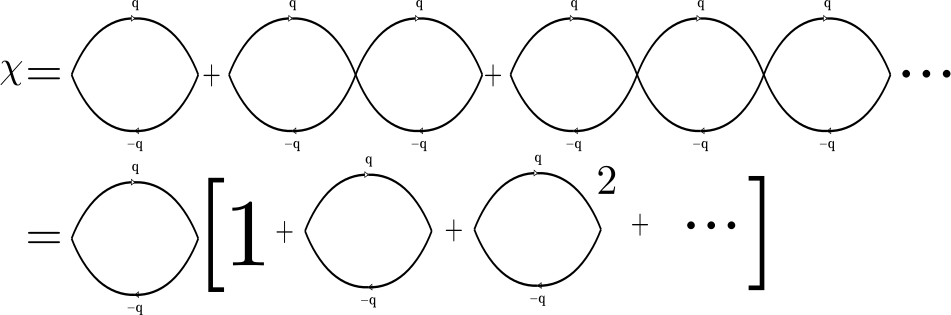
\includegraphics[scale=0.2]{./figures/term11.png}
\captionof{figure}{Susceptibility for Fermi liquid to all orders - geometric series}
\label{susc}
\end{center}
\subsection{BCS instability}
In the previous section we had ignored the functions \(V_2\) in our analysis, and that led us to the Fermi liquid picture. To make better contact with the BCS instability, we can include phonons into our picture. The electron-phonon interaction term is of the form
\begin{equation}\begin{aligned}
\int d\omega \int d\mathbf{k_1}\mathbf{k_2}dq\;g(\mathbf{k_1},\mathbf{k_2},\mathbf{q})\psi_{\mathbf k_2,\sigma}^\dagger \mathbf{R}(q) \psi_{\mathbf k_1,\sigma}
\end{aligned}\end{equation}
\(\mathbf{R}(q)\) is the canonical position variable for the phonons. Integrating out the phonons leaves us with a four-fermion interaction term of the form we have already considered before. Call this new interaction \(V_{ep}\). At the Debye energy \(E_D\), this coupling becomes of order unity. Also assume there's a coupling \(V_{ee}\) from the set \(\tilde V_{2,m}\) that grows under renormalization. At \(E = E_D\), this coupling becomes
\begin{equation}\begin{aligned}
	V_{ee}^* = V_{ee}\left(1 + \frac{V_{ee}}{4\pi}\ln \frac{E_0}{E_D}\right)^{-1}
\end{aligned}\end{equation}
The net interaction at the Debye energy is described by the coupling \(V_{ee}^* + V_{ep}\). There are two possibilities:
\begin{itemize}
	\item \(V_{ee}^* + V_{ep} > 0\): The total coupling will then shrink under the RG flow and decay to zero. This will lead to the Fermi liquid picture.
	\item \(V_{ee}^* + V_{ep} < 0\): \textbf{This will lead to the total coupling growing to large negative values at lower energies \(E < E_D\).} In this case, let the total coupling starting at \(E = E_D\) be \(\mathcal{V} = -|V_{ee}^* + V_{ep}|\). This total coupling will go as
		\begin{equation}\begin{aligned}
			|\mathcal{V}(E)| = |\mathcal{V}|\left(1 + \frac{|\mathcal{V}|}{4\pi}\ln \frac{E}{E_D}\right)^{-1}
		\end{aligned}\end{equation}
		Since \(\frac{|\mathcal{V}|}{4\pi} \sim O(1)\), the denominator is maximum at \(E = E_D\). The magnitude of the new coupling, \(|\mathcal{V(E)}|\), will diverge at a temperature \(E^*\) given by
		\begin{equation}\begin{aligned}
		1 + \frac{|\mathcal{V}|}{4\pi}\ln \frac{E^*}{E_D} = 0 \implies E^* = E_D e^{\frac{4\pi}{|\mathcal{V}|}} = E_D e^{-\frac{4\pi}{V_{ee}^* + V_{ep}}}
		\end{aligned}\end{equation}
\end{itemize}
\textbf{This energy scale signifies the onset of the BCS instability.}

\subsection{Treatment of Hubbard-like interaction in presence of nesting}

\begin{minipage}{270pt}
	Nesting is the term given to the phenomenon in which a single reciprocal lattice vector connects large parts of the Fermi surface. In other words, there exits a momentum \(\mathbf{Q}\) which satisfies
\begin{equation}\begin{aligned}
\mathbf{Q} \in \text{RLS}, \text{ and } E(\mathbf{K}) = -E(\mathbf{K+Q})
\end{aligned}\end{equation}
for a large number of \(\mathbf{K}\). These are the conditions under which a state \(\mathbf{K}\) can scatter to a state \(\mathbf{K+Q}\) in the presence of a periodic lattice. RLS stands for reciprocal lattice space.
\end{minipage}
\hspace*{20pt}
\begin{minipage}{250pt}
\begin{center}
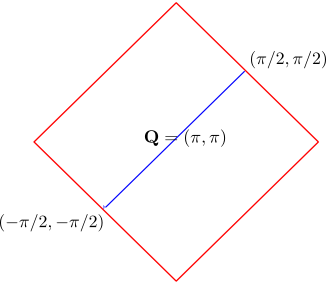
\includegraphics[scale=0.25]{./figures/term12.png}
\captionof{figure}{Nesting at Fermi surface}
\label{susc1}
\end{center}
\end{minipage}
 
The way this affects the RG calculation is as follows: While analyzing the tree-level RG flow of the four-Fermion interaction, we found a very strict criterion for exactly which of the momenta combinations survive the renormalization. The need to do that arose from the fact that even if the first three momenta lie within \([-\Lambda,\Lambda]\), the fourth one might note. The presence of the momentum \(\mathbf{Q}\) eases this restriction. If we define \(\mathbf{k_3} - \mathbf{k_1} = \mathbf{Q}\), then 
\begin{equation}\begin{aligned}
E(\mathbf{k_4}) = E(\mathbf{Q + k_2}) = -E(\mathbf{k_2)}
\end{aligned}\end{equation}
Thus, if \(\mathbf{k_2}\) lies within the allowed region, so will \(\mathbf{k_4}\). This means that all scatterings connected by \(\mathbf{Q}\) will now be marginal under the RG. 
 
We next consider such scatterings at one loop. Previously, we had seen that most of the diagrams vanished because either the poles were on the same half or the transfer momentum was so large that the allowed region was too small. In the present case, consider two virtual particles with momenta \(\mathbf{K}\) and \(\mathbf{K+Q}\), similar to what we considered previously. In the presence of nesting, the energies corresponding to these momenta are \(E(\mathbf{K})\) and \(E(\mathbf{K+Q}) = -E(\mathbf{K})\). Thus, if \(\mathbf{K}\) is a particle at \(\pm \Lambda\), then \(\mathbf{K+Q}\) can be a hole at \(\mp \Lambda\). The poles will then be on opposite halves and the integral will not vanish.
 
\textbf{We can hence conclude that this RG procedure can also be used to analyze the instabilities arising from a nested Fermi surface. Whether it gives the correct fixed points or not can be definitely concluded only by performing the calculation all the way.}
\end{document}
